\chapter{Background on Probabilistic Reasoning}
\label{chap:probabilistic}
%\chapter{Einleitung}
%\label{sec:einleitung}

This chapter discusses two mathematical frameworks for sequential decision making in stochastic environments. Section \ref{sec:MDP} covers the Markov decision process (MDP) in which the agent's interaction with the world is modeled as a discrete time stochastic process, where an agent chooses an action at each timestep. It is assumed that the state of the system is known at all times. In Subsection \ref{subsec:VALUEIT} the Value Iteration algorithm is presented, which computes the optimal action for each state.\\

In Section \ref{sec:POMDP} the partially observable Markov decision process (POMDP) is introduced, which generalizes the MDP to allow for unknown states. In addition to choosing an action, the agent collects an observation at each timestep, which allow it to reason about the current state of the system. Subsection \ref{subsec:SARSOP} briefly outlines SARSOP, a state-of-the-art algorithm for solving POMDPs.  
%%%%%%%%%%%%%%%%%%%%%%%%%%%%%%%%%%%%%%%%%%%%%%%%%%%%%%%%%%%%%%%%%%%%%%%%%%%%%%%%
%%%%%%%%%%%%%%%%%%%%%%%%%%%%%%%%%%%%%%%%%%%%%%%%%%%%%%%%%%%%%%%%%%%%%%%%%%%%%%%%
%%%%%%%%%%%%%%%%%%%%%%%%%%%%%%%%%%%%%%%%%%%%%%%%%%%%%%%%%%%%%%%%%%%%%%%%%%%%%%%%
%%%%%%%%%%%%%%%%%%%%%%%%%%%%%%%%%%%%%%%%%%%%%%%%%%%%%%%%%%%%%%%%%%%%%%%%%%%%%%%%
\section{Markov Decision Process}\label{sec:MDP}
Markov decision processes are used in various applications and fields like robotics, finances, population harvesting \cite{MDPsurvey} etc. In the field of robotics they are usually deployed as high-level planners. 
%%%%%%%%%%%%%%%%%%%%%%%%%%%%%
\subsection{Standard Formulation}\label{subsec:MDPFormulation}
Formally, a Markov decision process is a discrete time infinite horizon stochastic control process defined by the tuple $M = \langle \mathcal{S}, \mathcal{A}, T, R, \gamma \rangle$, where $\mathcal{S}$ is the discrete space of reachable states, $\mathcal{A}$ is the discrete space of actions, $T$ and $R$ are the transition and reward model and $\gamma \in [0,1]$ is the discount factor which determines how much future time steps are valued. At each time step the agent is in a state $s\in\mathcal{S}$, chooses an action $a\in\mathcal{A}$, receives a reward $R(s,a)$ and transitions according to $T(s,a,s')$ to a state $s'$.\\

In the standard formulation the following two assumptions are made:
\begin{enumerate}[(i)]
    \item\label{MDPass:i} The state $s$ is known at every time step.
    \item\label{MDPass:ii} Given state $s$ and action $a$, the MDP is conditionally independent of all previous states and actions.
\end{enumerate}
Assumption (\ref{MDPass:ii}) is called the \textit{Markov property} from which follows that the probability of ending up in  state $s'$ is only dependent on $s$ and $a$ of the current time step. This gives rise to the transition model $T:\mathcal{S}\times\mathcal{A}\times\mathcal{S}\rightarrow [0,1]$ which describes the probability that the agent transitions within one time step to state $s'$ if it chooses action $a$ in state $s$, i.e., $T(s,a,s')=P(s'|s,a)$. Note that if an action $a\in\mathcal{A}$ is not available in state $s$ the transition probability $T(s,a,s')$ is zero for all $s'\neq s$ and one for $s'=s$. 
Since the agent has to end up in a state it must hold that:
%
\begin{equation}
    \sum_{s'\in\mathcal{S}}pP(s'|a,s)=\sum_{s'\in\mathcal{S}}T(s,a,s')=1.
\end{equation}
%
The reward model $R:\mathcal{S}\times\mathcal{A}\rightarrow \mathbb{R}$ maps each state-action pair to a scalar, bounded reward. In other words, the agent receives the reward $R(s,a)$ for being in state $s$ and choosing action $a$.\\

The agent's goal is to maximize the \textit{expected return} by finding the optimal policy $\pi^*(s)$. A policy $\pi(s)$ is a unique mapping from state $s$ to action $a$, i.e., a function telling the agent which action to choose in each state. The expected return starting from state $s_\tau$ under a policy $\pi$ is called the value $V^\pi(s_\tau)$ of a state and given by:
%
\begin{equation}\label{eq:Vofpi}
    V^\pi(s) = \mathbb{E}\left[\sum_{k=0}^\infty \gamma^k\cdot r_{\tau+k}|s_\tau=s, \pi\right]
\end{equation}
%
where $r_{\tau+k}$ is the expected reward at time step $\tau+k$. 
The optimal policy $\pi^*$ is the policy with associated maximal value $V^*=V^{\pi^*}$ and is defined as:
%
\begin{equation}\label{eq:Vstar}
    \pi^*(s)=\underset{\pi}{\text{arg max }}V^\pi(s).
\end{equation}
%
In order for the MDP to be well defined, the value function needs to be bounded. This requires either choosing $\gamma<1$ or the presence of a set of terminal states $\mathcal{S}_t$. If the agent is in a terminal state $s_t$ it receives zero reward for all future actions and won't be able to leave the terminal state again. This is formalized with the following conditions on a terminal state:
%
\begin{align}
    R(s_t, a) &= 0 \quad \forall a\in\mathcal{A}\\
    T(s_t, a, s') &=  \begin{cases}1, & \text{if }s'=s_t;\\0, & \text{otherwise}.\end{cases}
\end{align}
%

    



%%%%%%%%%%%%%%%%%%%%%%%%%%%%%%%%%%%%%%%%%%%%%%%%%%%%%%%%%%%%%%%%%%%%%%%%%%%%%%%%
%%%%%%%%%%%%%%%%%%%%%%%%%%%%%%%%%%%%%%%%%%%%%%%%%%%%%%%%%%%%%%%%%%%%%%%%%%%%%%%%

\subsection{MDP Solving with Value Iteration}\label{subsec:VALUEIT}

By using the \textit{principle of optimality} \cite{dynprog} and using the transition and reward model, Equations \ref{eq:Vofpi} and \ref{eq:Vstar} can be reformulated in a recursive form known as the \textit{Bellman Equation}:
%
\begin{equation}\label{eq:BE}
    \begin{aligned}[t]
    V^*(s) &= \underset{a\in\mathcal{A}}{\text{max }} \underset{(s'|s)}{\mathbb{E}}\left[R(s,a) + \gamma\cdot V^*(s')|s, \pi \right]\\
    &= \underset{a\in\mathcal{A}}{\text{max }} \left(R(s,a) + \gamma\cdot \sum_{s'\in\mathcal{S}}\left(T(s,a,s')V^*(s')\right)\right).
    \end{aligned}
\end{equation}
%
Given the optimal value function $V^*(s)$ the optimal action $\pi^*(s)$ in state $s$ can be obtained by finding the action that maximizes the expected return:
\begin{equation}\label{eq:pistar}
    \pi^*(s) = \underset{a\in\mathcal{A}}{\text{arg max}}\left(R(s,a) + \gamma\cdot \sum_{s'\in\mathcal{S}}\left(T(s,a,s')V^*(s')\right)\right).
\end{equation}
The value iteration algorithm shown in Algorithm \ref{code:valueit} is an iterative method that aims to find the optimal value function $V^*(s)$ given the transition and reward model. In the first iteration, the value function $V_0(s)$ can be arbitrarily initialized for all $s\in\mathcal{S}$. In each iteration all values are updated using the Bellman update:
%
\begin{equation}\label{eq:VI}
    V_{k}(s) = \underset{a\in\mathcal{A}}{\max}  \left(R(s,a) + \gamma\cdot \sum_{s'\in\mathcal{S}}\left(T(s,a,s')V_{k-1}(s')\right)\right).
\end{equation}
%
Finding the optimal value generally takes infinite iterations. There is a termination criteria defined on the maximal change in value from iteration $k-1$ to $k$. Finally, the optimal policy is extracted by applying Equation \ref{eq:pistar}. Note that other popular solving methods exist like policy iteration or linear programming \cite{dynprog}.
%
\begin{algorithm}[htb!]
    \DontPrintSemicolon
    \caption{Value Iteration}
    \label{code:valueit}
    \SetKwInOut{Input}{input}
    \SetKwInOut{Output}{output}
    \Input{threshold $\epsilon$}
    \Output{$\pi^*$}
         $V_0(s) = \max_{a\in\mathcal{A}} R(s,a)$    \tcp*[r]{initialize value function}
         $V_1 \leftarrow$ equation \ref{eq:VI} $\forall s\in\mathcal{S}$ \tcp*[r]{bellman update}
            \While{ $\underset{s\in\mathcal{S}}{\max }||V_k(s)-V_{k-1}(s)||_\infty < \epsilon$}{
            $V_{k+1} \leftarrow$ equation \ref{eq:VI} $\forall s\in\mathcal{S}$ \tcp*[r]{bellman update}
        }
        $\pi^*(s) \leftarrow$ equation \ref{eq:pistar} $\forall s\in\mathcal{S}$ \tcp*[r]{extract optimal policy}
\end{algorithm}
%

%%%%%%%%%%%%%%%%%%%%%%%%%%%%%%%%%%%%%%%%%%%%%%%%%%%%%%%%%%%%%%%%%%%%%%%%%%%%%%%%
%%%%%%%%%%%%%%%%%%%%%%%%%%%%%%%%%%%%%%%%%%%%%%%%%%%%%%%%%%%%%%%%%%%%%%%%%%%%%%%%

%%%%%%%%%%%%%%%%%%%%%%%%%%%%%%%%%%%%%%%%%%%%%%%%%%%%%%%%%%%%%%%%%%%%%%%%%%%%%%%%
%%%%%%%%%%%%%%%%%%%%%%%%%%%%%%%%%%%%%%%%%%%%%%%%%%%%%%%%%%%%%%%%%%%%%%%%%%%%%%%%
%%%%%%%%%%%%%%%%%%%%%%%%%%%%%%%%%%%%%%%%%%%%%%%%%%%%%%%%%%%%%%%%%%%%%%%%%%%%%%%%
%%%%%%%%%%%%%%%%%%%%%%%%%%%%%%%%%%%%%%%%%%%%%%%%%%%%%%%%%%%%%%%%%%%%%%%%%%%%%%%%
\section{Partially Observable MDPs}\label{sec:POMDP}
The partially observable Markov decision process is as its name suggests an extension of the Markov decision process. Whereas a MDP assumes that the state $s$ of the system is known (assumption (\ref{MDPass:i})), a POMDP does not have direct access to the state. Instead, at each time step an observation is made, which can be used to reason about the current state using a sensor/observation model. This reasoning about the current state is done by keeping track of the belief of the states.
\subsection{Standard Formulation}
Formally, a POMDP is defined by the tuple $P = \langle \mathcal{S}, \mathcal{A}, \mathcal{O}, T, Z, R, b_0, \gamma \rangle$, where $\mathcal{O}$ is a discrete set of observation, $Z$ is the observation model, $b_0$ is the initial belief of the state and $\mathcal{S}, \mathcal{A}, T, R, \gamma$ are identical to the MDP definition in Subsection \ref{subsec:MDPFormulation}. In each time step the agent is in a state $s\in\mathcal{S}$, chooses an action $a\in\mathcal{A}$, receives a reward $R(s,a)$, transitions according to $T(s,a,s')$ to state $s'$ and then receives an observation $o$ according to $Z(o, s', a)$. See Figure \ref{fig:POMDP} for a graphical representation of a POMDP.\\ 

The observation model $Z:\mathcal{O}\times\mathcal{S}\times\mathcal{A}\rightarrow [0, 1]$ describes the probability that the agent makes observation $o$ given that it transitioned to state $s'$, i.e., $Z(o,s',a) = P(o|s',a)$. Since the agent receives an observation after every time step, it must hold that:
\begin{equation}
    \sum_{o\in\mathcal{O}}P(o|s',a) = \sum_{o\in\mathcal{O}}Z(o,s', a) = 1.
\end{equation}

\begin{figure}
    \centering
    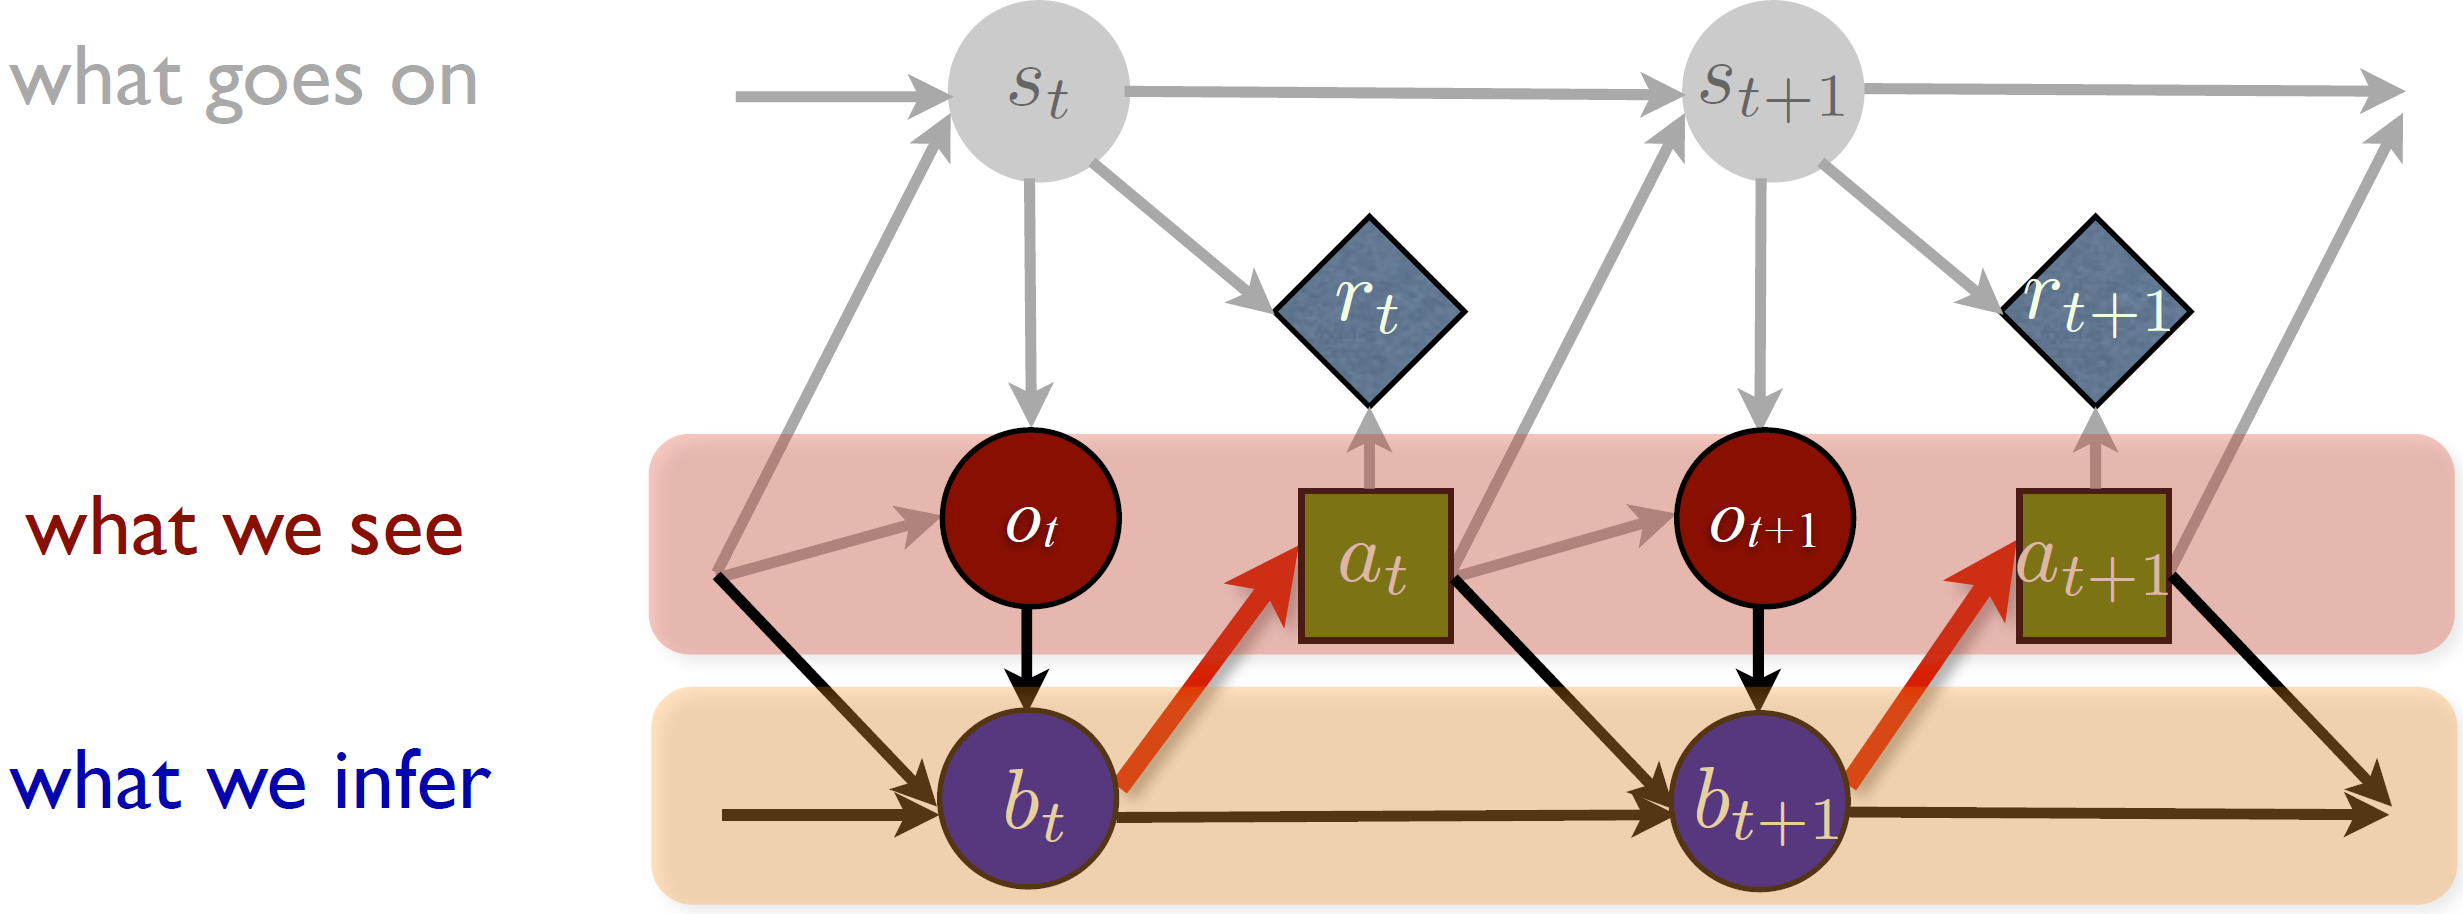
\includegraphics[width=\textwidth]{Report/images/POMDP.png}
    \caption{Visualisation of a time step in a POMDP. Copied from David Hsu, 2016 \cite{POMDPpresi}}
    \label{fig:POMDP}
\end{figure}


The initial belief $b_0:\mathcal{S}\rightarrow [0, 1]$ is a distribution of state $s$ and represents the belief/probability that the agent is in state $s$. Note that since the agent has to be in a state the summation of the belief of all states must be equal to one:
\begin{equation}\label{eq:b0norm}
    \sum_{s\in\mathcal{S}} b_0(s)=1.
\end{equation}
The initial belief $b_0(s)$ can be propagated to the next time step using the transition and observation model. The belief $b'(s')$ of being in state $s'$ after making observation $o$ and choosing action $a$ can be written as:
%
\begin{equation}\label{eq:bdash}
    \begin{aligned}[t]
    b'(s') &= \eta \cdot P(o|s', a)\cdot \sum_{s\in\mathcal{S}}P(s'|s,a)\cdot b(s) \\
    &=\eta \cdot Z(o,s',a)\cdot \sum_{s\in\mathcal{S}}T(s,a,s')\cdot b(s)
    \end{aligned}
\end{equation}
%
where $\eta$ is the normalization constant, s.t. Equation \ref{eq:b0norm} holds.\\

The Bellman equation can be formalized similarly to the MDP case (Equation \ref{eq:BE}) by defining the value function on beliefs instead of states and taking possible observations into account. For this purpose the probability of observing $o$ after choosing $a$ in belief $b$ is derived:
%
\begin{align}
    P(o|b,a) &= \sum_{s'\in\mathcal{S}}P(o,s'|b,a)\\
    &= \sum_{s'\in\mathcal{S}}P(o|s',b, a)\cdot P(s'|b, a)\\
    &=\label{eq:line2} \sum_{s'\in\mathcal{S}}P(o|s', a)\cdot P(s'|b, a)\\
    &=\label{eq:line3}  \sum_{s'\in\mathcal{S}}\left(P(o|s', a)\cdot \sum_{s\in\mathcal{S}}\left(P(s'|a,s)\cdot b(s)\right)\right)\\
    &= \sum_{s'\in\mathcal{S}}\left(Z(o,s', a)\cdot \sum_{s\in\mathcal{S}}\left(T(s,a,s')\cdot b(s)\right)\right)
\end{align}
%
where in \ref{eq:line2} the conditional independence of $o$ and $b$ given $s'$ is used. Now the Bellman equation for POMDPs can be formalized as:
%
\begin{equation}\label{eq:BEPOMDP}
    V^*(b) = \underset{a\in\mathcal{A}}{\max}\left( R(b,a) + \gamma\cdot \sum_{o\in\mathcal{O}} P(o|b,a)V^*(b') \right).
\end{equation}
%
where $b'$ is given by Equation \ref{eq:bdash}. $R(b,a)$ is the reward of choosing action $a$ in belief $b$ and is computed as a linear combination of the reward model:
%
\begin{equation}\label{eq:R_b}
    R(b,a) = \sum_{s\in\mathcal{S}}R(s,a)\cdot b(s).
\end{equation}
%
With the formulation of \ref{eq:BEPOMDP} the POMDP is written as a MDP where the state is replaced by the belief $b$, the reward model is given by $R(b,a)$ and the transition model by $P(o|b,a)$.\\

One key difference between a standard MDP and Equation \ref{eq:BEPOMDP} is that the state $s$ is a finite discrete valued variable while the belief $b$ is a continuous valued variable. Thus, the value iteration algorithm from Subsection \ref{subsec:VALUEIT} cannot directly be applied.\\

There is an adapted value iteration algorithm for POMDPs that builds on the idea of \textit{conditional plans} and their associated \textit{utilities}. A conditional plan $p$ considers which action to choose after each possible observation and can be thought of as a decision tree where the nodes are actions and the edges are observations.
The utility $\alpha_p(s)$ is the return for executing a fixed conditional plan $p$ in state $s$. It can be recursively computed as:
\begin{equation}\label{eq:POMDP_valit}
    \alpha_p(s) = R(s,a) + \gamma\left(\sum_{s'\in\mathcal{S}}T(s,a,s')\sum_{o\in\mathcal{O}}Z(o, s', a)\alpha_{p.o}(s')\right)
\end{equation}
where $p.o$ is the subtree of $p$ after the first observation $o$. The \textit{expected utility} of executing $p$ with belief $b$ is equivalent to the value of belief b:
\begin{align}
        V_p(b) &= \sum_{s\in\mathcal{S}}b(s)\cdot \alpha_p(s)\\
        &=\label{eq:b_alpha} b\cdot \alpha_p
\end{align}
where $b$ and $\alpha_p$ are treated as vectors in \ref{eq:b_alpha}. The optimal policy is to execute the plan $p$ with highest utility $\alpha_p(s)$. While there are an infinite number of plans, the optimal value function can be approximated arbitrarily close by the following convex, piecewise-linear function:
%
\begin{equation}\label{eq:Vstarbalpha}
    V^*(b) \approx \max_{\alpha\in\Gamma} b\cdot \alpha
\end{equation}
%
where $\Gamma$ is a finite set of $\alpha$-vectors. The value function corresponds to a hyperplane in belief space.\\

The adapted value iteration algorithm starts with all possible plans $p$ of depth one and their associated utilities. In each iteration the plans are continued one time step further and the utilities are updated according to \ref{eq:POMDP_valit}. Plans that are suboptimal across the entire belief space are pruned. This process is repeated until the change in the value function (Equation \ref{eq:b_alpha}) is smaller than a user-defined threshold.\\

This na\"ive implementation of value iteration is infeasible for real problems, as it can be shown that the time complexity of such a method is exponential in both the number of observations and the number of actions. More recent POMDP solvers build upon the idea of $\alpha$-vectors to approximate the value function and combine it with belief space sampling.
%%%%%%%%%%%%%%%%%%%%%%%%%%%%%%%%%%%%%%%%%%%%%%%%%%%%%%%%%%%%%%%%%%%%%%%%%%%%%%%%
%%%%%%%%%%%%%%%%%%%%%%%%%%%%%%%%%%%%%%%%%%%%%%%%%%%%%%%%%%%%%%%%%%%%%%%%%%%%%%%%
\subsection{SARSOP}\label{subsec:SARSOP}
Sarsop \cite{6284837} is a state-of-the-art point-based POMDP solver. It approximates the optimal value function through $\alpha$-vectors and uses a sampling tree. 
Instead of sampling the entire belief space $\mathcal{B}$, Sarsop aims at sampling the \textit{optimally reachable belief space} $\mathcal{R}^* \subset \mathcal{B}$.
The optimally reachable belief space is the subset of beliefs which can be reached by following the optimal policy $\pi^*(b)$. This subset is for most problems much smaller than the entire belief space and thus accelerates the solving process.\\

A sampling tree is constructed with the initial belief point $b_0$ as root. An upper and lower bound of the value function is used to prune suboptimal branches. The upper value is initialized by considering the optimal MDP policy of the problem. For the lower bound the best fixed-action policy can be used. The tree is propagated by sampling action-observation pairs from the belief points at the leaf nodes of the tree. The bounds are then iteratively improved with the value update from Equation \ref{eq:POMDP_valit}. Branches of the tree that are not in between the upper and lower bounds are pruned. This way the sampled tree stays close to the optimally reachable belief space. Sarsop terminates either when the gap between upper and lower bound is smaller than a defined threshold or after the termination time is reached.\\

Sarsop is available for download at \url{https://bigbird.comp.nus.edu.sg/pmwiki/farm/appl/}. The input of the algorithm is the POMDP definition encoded in an xml file and the output is an xml file containing the set of $\alpha$-vectors. The optimal action to execute for belief $b$ can be extracted using Equation \ref{eq:Vstarbalpha}. 


%%%%%%%%%%%%%%%%%%%%%%%%%%
